\chapter{Resultados}
\label{chapter:Resultados}

\section{Testes unitários}

Durante todo o desenvolvimento do SocialFramework foi eleborado uma suíte de testes para tentar garantir que cada ponto do código funcione da devida maneira. Desse modo, o desenvolvedor pode inserir novos códigos, módulos ou alterar um código existente, com mais tranquilidade e sabendo que o restante de código irá funcionar adequadamente. Caso algum resultado esperado seja diferente do obtido a suite de testes irá apontar a falha.

Para a realização dos testes foi utilizada a \textit{gem} do Rspec, essa \textit{gem} é amplamente utilizada pela comunidade do Rails. E para a visualizar o relatório de testes foi utilizado o Code Climate, que é uma ferramenta online que realiza uma análise estática do código fonte, atualmente é suportado as linguagens: Ruby, Python, JavaScript e PHP.

No inico do desenvolvimento foi estabelecido uma meta de que se deveria testar no mínimo 90\% do código fonte. Fui comprida essa meta obtendo-se 97\% de cobertura do código, porém essa métrica não corresponde a realidade. pois os arquivos ``elements\_factory.rb'', ``elements\_factory\_default.rb'' e ``graph\_elements.rb'' tiveram a cobertura, respectivamente, de 60\%, 80\% e 84\%, diminuindo a cobertura real do código fonte, entretando esses arquivos possuem classes ``abstratas'' e deveriam ser desconsiderados. Porém, em Ruby não existe o conceito de classe abstrata, porém Olsen apresenta uma abordagem de se obter esse conceito em seu livro \cite{Olsen:2007}. Um exemplo dessa abordagem pode ser observada a seguir:

 \begin{lstlisting}[
    label=listing:classe_abstrata,
    caption=Classe abstrata,
    numbers=left,
    language=Ruby,
    basicstyle=\footnotesize\sffamily,
    keywordstyle=\color{red},
    stringstyle=\color{blue},
]
# Define abstract methods to Vertex
class Edge
  attr_accessor :origin, :destiny, :labels
  
  # Constructor to Edge
  # ====== Params:
  # +origin+:: +Vertex+ relationship origin
  # +destiny+:: +Vertex+ relationship destiny
  # Returns NotImplementedError
  def initialize origin, destiny
    raise 'Must implement method in subclass'
  end
end
\end{lstlisting}

A seguir é apresentado na Figura \ref{Cobertura_teste} cada arquivo e sua cobertura.

\begin{figure}[!h]
	\centering
	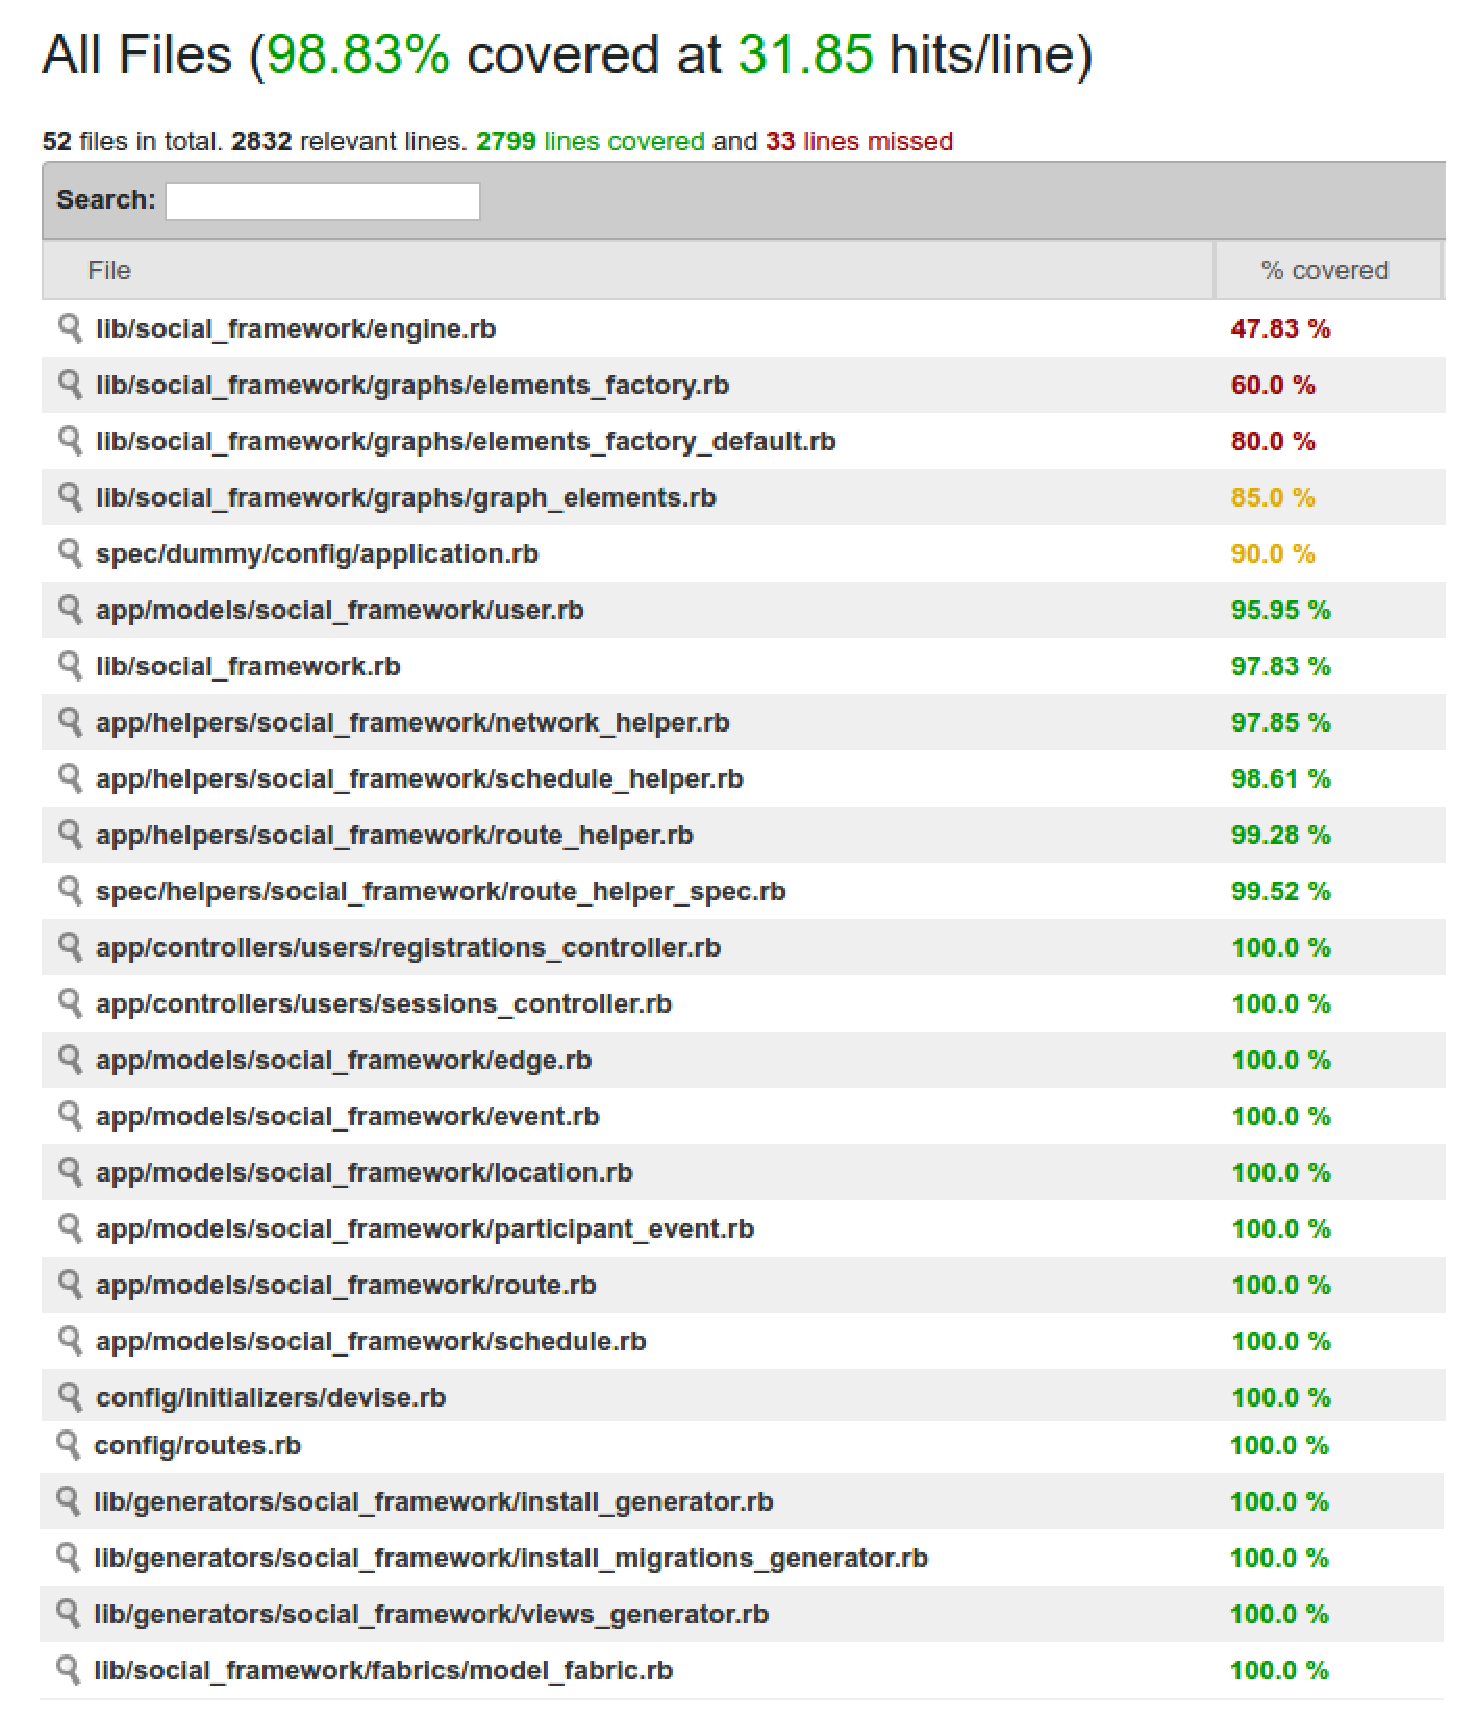
\includegraphics[scale=0.55]{figuras/capitulo7/cobertura.eps}
	\caption[Cobertura de teste]{Cobertura de teste}
	\label{Cobertura_teste}
\end{figure}

\section{Relatório de desempenho}

Após a verificação do correto fluxo que o \textit{framework} executa, foi realizado testes de desempenho do mesmo, analisando o tempo de processamento e o consumo de memória.

% \subsecton{Tempo de execução}

% \subsecton{Memória}
% falar se é linear

\section{Qualidade do SocialFramework}

Essa seção irá evidenciar o resultado da qualidade do código fonte do \textit{framework}. A partir da análise de código fonte realizada pela ferramenta Code Climate foi possível obter as métricas e realizar uma análise qualitatica dos resultados obtidos.

Medir e monitorar a qualidade do software é fundamental. Mesmo uma ótima suíte de testes pode produzir informações apenas sobre características externas, não refletindo qualidades como manutenabilidade, modularidade, flexibilidade e simplicidade \cite{Filho:2013}.

Filho afirma ainda que nem tudo vale a pena controlar. Portanto, não se deve procurar medir tudo, mas escolher bem as métricas para avaliar e controlar o projeto \cite{Filho:2013}.

As métricas que foram monitoradas durante o projeto foram:

\begin{enumerate}
	\item \textbf{Complexidade}: Essa métrica fornece uma análise da complexidade e do esforço gasto em um trecho de código. Para isso é utilazado as seguintes métricas;
	\begin{enumerate}
		\item \textbf{Complexidade ciclomática}: é calculada pela quantidade de caminhos que é possível percorrer no método. Dessa forma, sempre começa em 1, pois todo método tem pelo menos um caminho possível. Para cada estrutura condicional ou repetitiva( if, unless, elsif, while, until, for, when, rescue ) é adicionado mais 1 para a complexidade;
		\item \textbf{Tamanho do código}: que é a quantidade de linhas que o código possui, desconsiderando comentários e espaços em branco;
		\item \textbf{Complexidade ABC}: o cálculo da complexidade é baseado em três pontos:
		\begin{enumerate}
			\item \textbf{Assignment}: qualquer atribuição explícita de um dado para uma variável, por exemplo: = *= /= \%= += <<= >>= \&= |= >= ++ —, etc;
		    \item \textbf{Branch}: quando um caminho fora do escopo do programa é feito, por exemplo: uma chamada de método de instância e/ou classe, um operador new instanciando uma classe, etc;
    		\item \textbf{Condition}: qualquer teste lógico/booleano, == != <= >= < > else case default try catch ? e condicionais unários.
		\end{enumerate}
	\end{enumerate}
	\item \textbf{Duplicação de código}: analiza a similaridade de trechos de código na aplicação. Para cada nível de similaridade, é atribuido um peso diferente, indo de similar até identico, resultando no número bruto que é a somatória de todos os arquivos. Espaços em branco, nomes de variáveis, métodos e classes são ignorados pela ferramenta;
	\item \textbf{Estilo}: Verifica se o projeto utiliza o guia de estilo descrito pela comunidade Rails. E aponta onde estão as más práticas relacionadas a padrões e convenções que não estão sendo respeitadas na aplicação;
	\item \textbf{Segurança}: Utiliza um \textit{fork} do Brakeman na versão 2.6.2 para identificar as vulnerabilidades do projeto Rails.
\end{enumerate}

\newpage

A partir dessas métricas o Code Climate realiza o cálculo do GPA (\textit{grade point average}) que é uma espécie de média de todos os arquivos do projeto, o GPA possui um intervalo de 0 a 4 pontos, levando em consideração as notas dos arquivos, que varia de `A' a `F'.Desse modo, no início do projeto foi estabelacio uma meta de 3 pontos. Essa meta foi atingida com exito, obtendo-se 3.29 pontos, como pode ser observado na Figura \ref{GPA}.

\begin{figure}[!h]
	\centering
	\includegraphics[scale=0.5]{figuras/capitulo7/gpa.eps}
	\caption[GPA]{GPA}
	\label{GPA}
\end{figure}

Esse valor do GPA foi obtido de acordo com a Tabela \ref{gpa_arquivos}, que ilustra a quantidade de arquivos com as notas de `A' até `F'.

\begin{table}[!h]
\centering
\caption{Nota de cada arquivo}
\label{gpa_arquivos}
\begin{tabular}{cccccc}
\toprule
\textbf{Nota A} & \textbf{Nota B} & \textbf{Nota C} & \textbf{Nota D} & \textbf{Nota E} & \textbf{Nota F} \\ \midrule
50 & 1 & 1 & 1 & 0 & 0							   \\ \bottomrule
\end{tabular}
\end{table}

\section{Uso da rede social}
